\documentclass[12pt]{article}
\usepackage[margin=2.5cm]{geometry}
\usepackage{enumerate}
\usepackage{amsfonts}
\usepackage{amsmath}
\usepackage{fancyhdr}
\usepackage{amsmath}
\usepackage{amssymb}
\usepackage{amsthm}
\usepackage{mdframed}
\usepackage{graphicx}
\usepackage{subcaption}
\usepackage{adjustbox}
\usepackage{listings}
\usepackage{xcolor}
\usepackage{booktabs}
\usepackage[utf]{kotex}
\usepackage{hyperref}

\definecolor{codegreen}{rgb}{0,0.6,0}
\definecolor{codegray}{rgb}{0.5,0.5,0.5}
\definecolor{codepurple}{rgb}{0.58,0,0.82}
\definecolor{backcolour}{rgb}{0.95,0.95,0.92}

\lstdefinestyle{mystyle}{
    backgroundcolor=\color{backcolour},
    commentstyle=\color{codegreen},
    keywordstyle=\color{magenta},
    numberstyle=\tiny\color{codegray},
    stringstyle=\color{codepurple},
    basicstyle=\ttfamily\footnotesize,
    breakatwhitespace=false,
    breaklines=true,
    captionpos=b,
    keepspaces=true,
    numbers=left,
    numbersep=5pt,
    showspaces=false,
    showstringspaces=false,
    showtabs=false,
    tabsize=1
}

\lstset{style=mystyle}

\pagestyle{fancy}
\renewcommand{\headrulewidth}{0.4pt}
\lhead{Hyungmo Gu}
\rhead{CSC369 Week 9 Notes}

\begin{document}
\title{CSC369 Week 9 Notes}
\author{Hyungmo Gu}
\maketitle

\section{Disk I/O}

\begin{itemize}
    \item File system implementation
    \begin{itemize}
        \item Files and directories live on \textbf{secondary storage}
        \begin{itemize}
            \item Anything outisde of ``Primary memory''
            \item Is persistent (or non-volatile): Data survives loss of power
        \end{itemize}
    \end{itemize}
    \item Disk components

    \begin{center}
        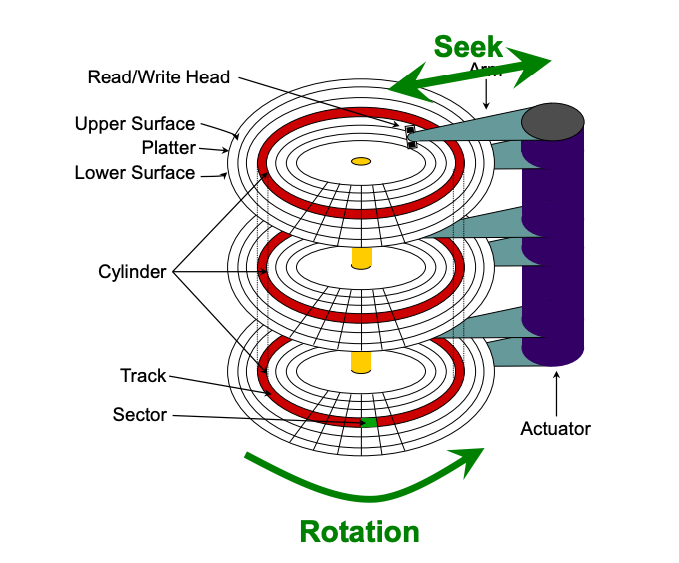
\includegraphics[width=0.6\linewidth]{../images/week_9_notes_1_1.png}
    \end{center}

    \begin{itemize}
        \item \textbf{Actuator:}
        \begin{itemize}
            \item is an electronic device controlled by a motor that moves the
            hard drive head arm. $^{[1]}$
        \end{itemize}

        \begin{center}
            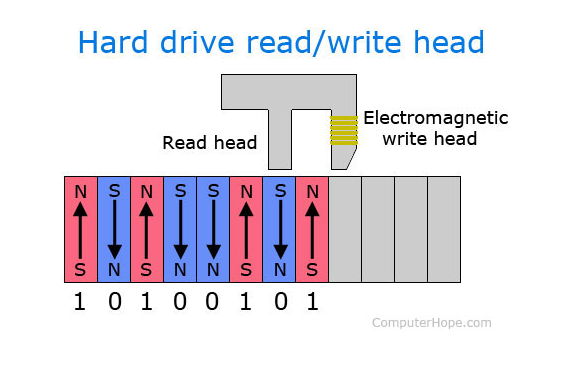
\includegraphics[width=0.5\linewidth]{../images/week_9_notes_1_2.png}
        \end{center}

        \item \textbf{Read/Write Heads:}
        \begin{itemize}
            \item are the small parts of a hard drive which move above the disk
            platter and transform the platter's magnetic field into electric current $^{[1]}$
        \end{itemize}
        \begin{center}
            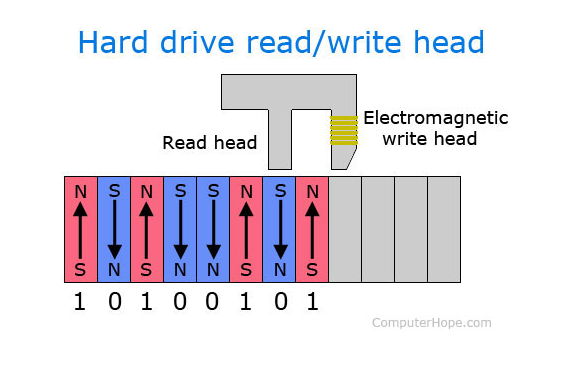
\includegraphics[width=0.8\linewidth]{../images/week_9_notes_1_3.png}
        \end{center}
        \item \textbf{Platter:}
        \begin{itemize}
            \item One or more aluminum, glass, or ceramic disk that
        is coated in a magnetic media $^{[1]}$
            \item All modern drives use glass or glass-ceramic platters $^{[2]}$
        \end{itemize}

        \begin{center}
            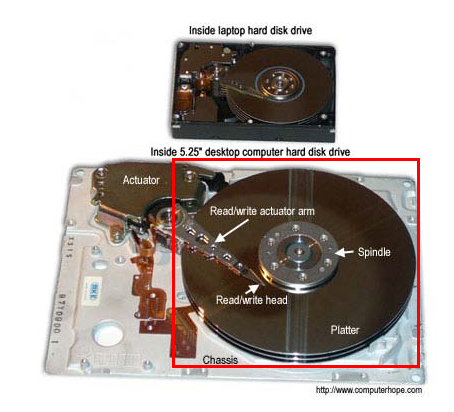
\includegraphics[width=0.5\linewidth]{../images/week_9_notes_1_4.png}
        \end{center}
        \item \textbf{Cylinder:}
        \begin{itemize}
            \item is any set of all tracks of equal diameter in a hard disk drive (HDD) $^{[3]}$
        \end{itemize}

        \begin{center}
            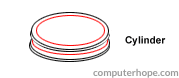
\includegraphics[width=0.4\linewidth]{../images/week_9_notes_1_5.png}
        \end{center}

        \item \textbf{Track:}
        \begin{itemize}
            \item is a data storage ring on a computer hard drive
        that is capable of storing information.
        \end{itemize}

        \begin{center}
            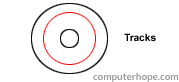
\includegraphics[width=0.4\linewidth]{../images/week_9_notes_1_6.png}
        \end{center}
        \item \textbf{Sector:}
        \begin{itemize}
            \item A division of storage medium on a hard drive
            that is a wedge shaped section of one of the circular tracks.
            \item Each arc is sector that \underline{usually holds 512 byte of data}.
        \end{itemize}

        \begin{center}
            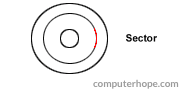
\includegraphics[width=0.4\linewidth]{../images/week_9_notes_1_7.png}
        \end{center}
    \end{itemize}

    \bigskip

    \underline{\textbf{Refernces:}}

    \bigskip

    \begin{enumerate}[1)]
        \item Computer Hope: Actuator, \href{https://www.computerhope.com/jargon/a/actuator.htm}{link}
        \item Etty94. (2016, August 1). \textit{Hard disk drive components}. Medium. \href{https://www.slideshare.net/Etty94/hard-disk-drive-components}{link}
        \item The Linux Information Project : Cylinder Definition, \href{http://www.linfo.org/cylinder.html}{link}
    \end{enumerate}

    % \item Disk service time
    % \item Mixing workloads can be tricky
    % \item Components of disk access time
    % \item Disk are slow
    % \item OS design principles
    % \item Disks are messy
    \item OS $\leftrightarrow$ disk interaction
    \begin{itemize}
        \item The old way
        \begin{itemize}
            \item Is called \textbf{Extended CHS} (Extended Cylinder, Head, Sector)
            \item Specifying disk requests requires a lot of info
            \begin{itemize}
                \item Cylinder \#, Surface \#, Track \#, Sector \#, transfer size $\cdots$
            \end{itemize}

            \item Modern disks are even more complicated
            \begin{itemize}
                \item Not all tracks have the same number of sectors
                \item Sectors are remapped
            \end{itemize}
            \item Older disks require OS to specify all of this
            \begin{itemize}
                \item The OS needs to know all disk parameters
            \end{itemize}
        \end{itemize}
        \item Now
        \begin{itemize}
            \item \textbf{Logical Block Addressing}
        \end{itemize}
    \end{itemize}

    \item Logical Block Addressing
    \begin{itemize}
        \item Is a common scheme used for specifying the location of blocks of data
        on computer storage device $^{[1]}$
        \item Is implemented in most hard disk drives after 1996 $^{[1]}$
        \item Hides disk parameters from the OS
        \item Exposes storage as linear array of blocks
        \begin{itemize}
            \item Maps blocks to cylinder/surface/track/sector
            \item Each block size is \underline{512 bytes}
        \end{itemize}
    \end{itemize}

    \begin{center}
        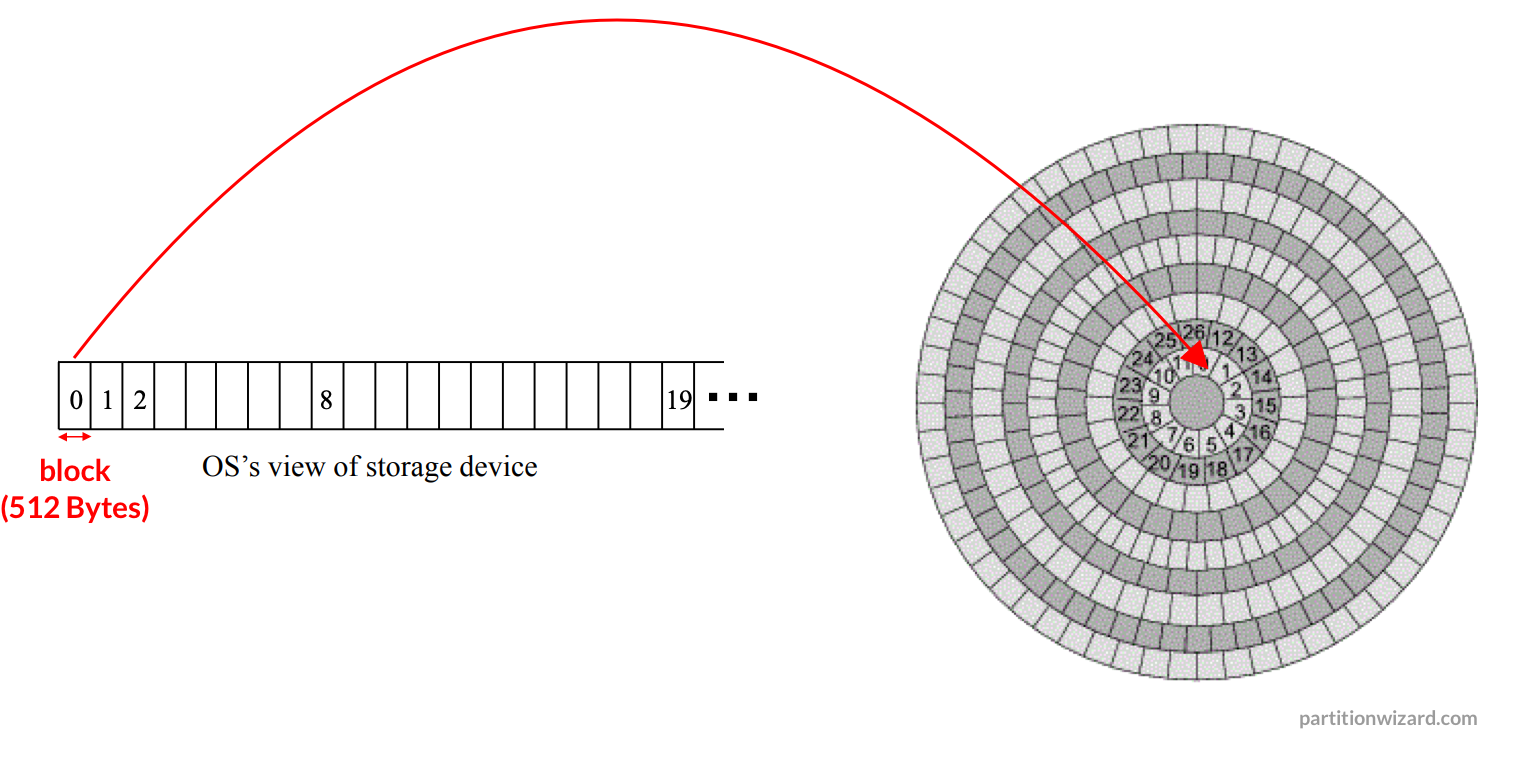
\includegraphics[width=0.8\linewidth]{../images/week_9_notes_1_8.png}
    \end{center}

    \bigskip

    \underline{\textbf{Refernces:}}

    \bigskip

    \begin{enumerate}[1)]
        \item Wikipedia: Logical Block Addressing, \href{https://en.wikipedia.org/wiki/Logical_block_addressing}{link}
    \end{enumerate}

    \item Disk Scheduling
    \begin{itemize}
        \item Is also known as I/O scheduling $^{[1]}$
        \item Is done by operating systems $^{[1]}$
        \item Is important because $^{[1]}$
        \begin{itemize}
            \item Hard drives are one of the slowest parts of the computer system
            and thus need to be accessed in an efficient manner
        \end{itemize}
    \end{itemize}

    \bigskip

    \underline{\textbf{Refernces:}}

    \bigskip

    \begin{enumerate}[1)]
        \item Geeks for Geeks: Disk Scheduling Algorithms, \href{https://www.geeksforgeeks.org/disk-scheduling-algorithms/}{link}
    \end{enumerate}
    % \item Back to Files and Directories
    % \item Disk Layout Strategies
    % \item Indexed Allocation: Unix Inodes
    % \item Unix Inodes and Path Search
    \item File System Implementation
    \begin{itemize}
        \item \textbf{Master Block / Super Block} determines location of root directory
        \item \textbf{Free map / Bitmap} determines which blocks are free, allocated
        \item Remaining disk blocks used to store files (and dirs)

        \begin{center}
            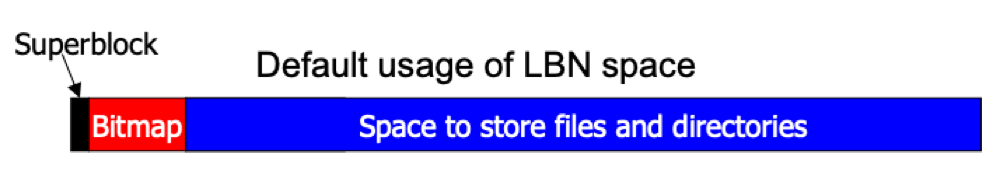
\includegraphics[width=0.8\linewidth]{../images/week_9_notes_1_9.png}
        \end{center}
    \end{itemize}

    \pagebreak

    \begin{mdframed}
        \underline{\textbf{Aside}}

        \bigskip

        \begin{itemize}
            \item LBN (Logical Block Number)
            \begin{itemize}
                \item Is the index of linear array of blocks
            \end{itemize}

            \begin{center}
                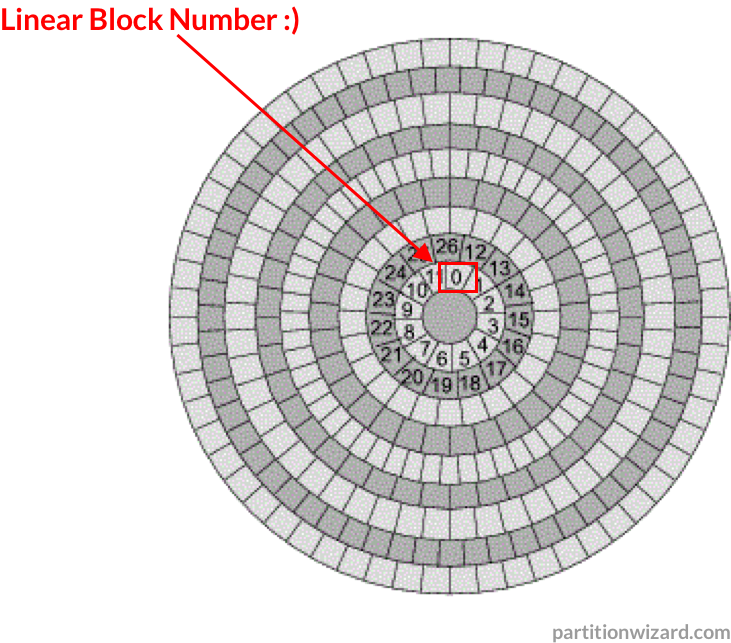
\includegraphics[width=0.8\linewidth]{../images/week_9_notes_1_10.png}
            \end{center}
        \end{itemize}
    \end{mdframed}
    % \item Original Unix File System
    % \item Data and Inode Placement
    \item FFS (Fast File System)
    \begin{itemize}
        \item Is an improvement made to original Unix File System
        \item Is done in early-mid 80s
        \item Improved disk utilization and decreased response time
        \item Uses \textbf{Cylinder Groups}
    \end{itemize}
    % \item Cylinder Groups
    % \item Space Allocation in Cylinder Groups
    % \item More FFS Solutions
    % \item FFS: Consistency I ssues
    % \item FFS Observation 1
    % \item FFS Observation 2
    \item Log Structured File System (LSF)
    \begin{itemize}
        \item Is file system designed to address exponentially improving
        CPU speed and slowly improving HDD speed. $^{[1]}$
    \end{itemize}

    \bigskip

    \underline{\textbf{Refernces:}}

    \bigskip

    \begin{enumerate}[1)]
        \item Ousterhout J. (1991). \textit{The Design and Implementation of a Log-Structured File System}. \href{https://people.eecs.berkeley.edu/~brewer/cs262/LFS.pdf}{link}
    \end{enumerate}
    \item NTFS (Windows)
    \begin{itemize}
        \item Is an acronym for \textbf{NT File System}
        \item Was first introduced in 1993, as part of Windows NT 3.1 Release $^{[1]}$
        \item Replaces traditional FAT (File Allocation Table) file system
        \item Is used in Windows NT, Windows 2000 and above $^{[1]}$
    \end{itemize}

    \begin{center}
        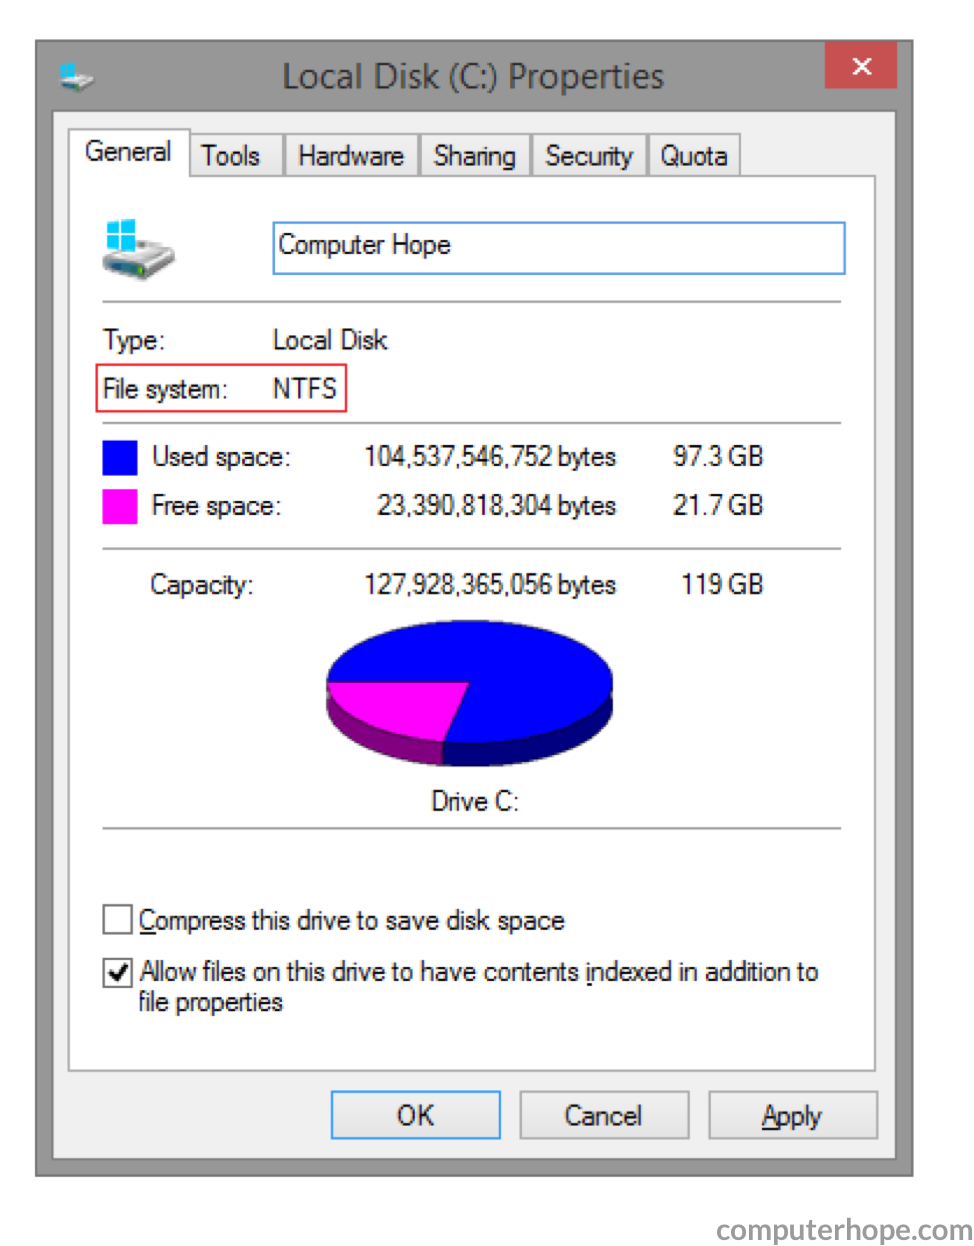
\includegraphics[width=0.8\linewidth]{../images/week_9_notes_1_11.png}
    \end{center}

    \bigskip

    \underline{\textbf{Refernces:}}

    \bigskip

    \begin{enumerate}[1)]
        \item Datto : What Is NTFS and How Does It Work?, \href{https://www.datto.com/library/what-is-ntfs-and-how-does-it-work}{link}
    \end{enumerate}
    \item MFT Record
    \begin{itemize}
        \item Is also called \textbf{Master File Table Record} $^{[1]}$
        \item Contains records about every other file and directory in NTFS volume $^{[1]}$
        \item Is a table of metadata like inodes but more flexible
    \end{itemize}

    \begin{center}
        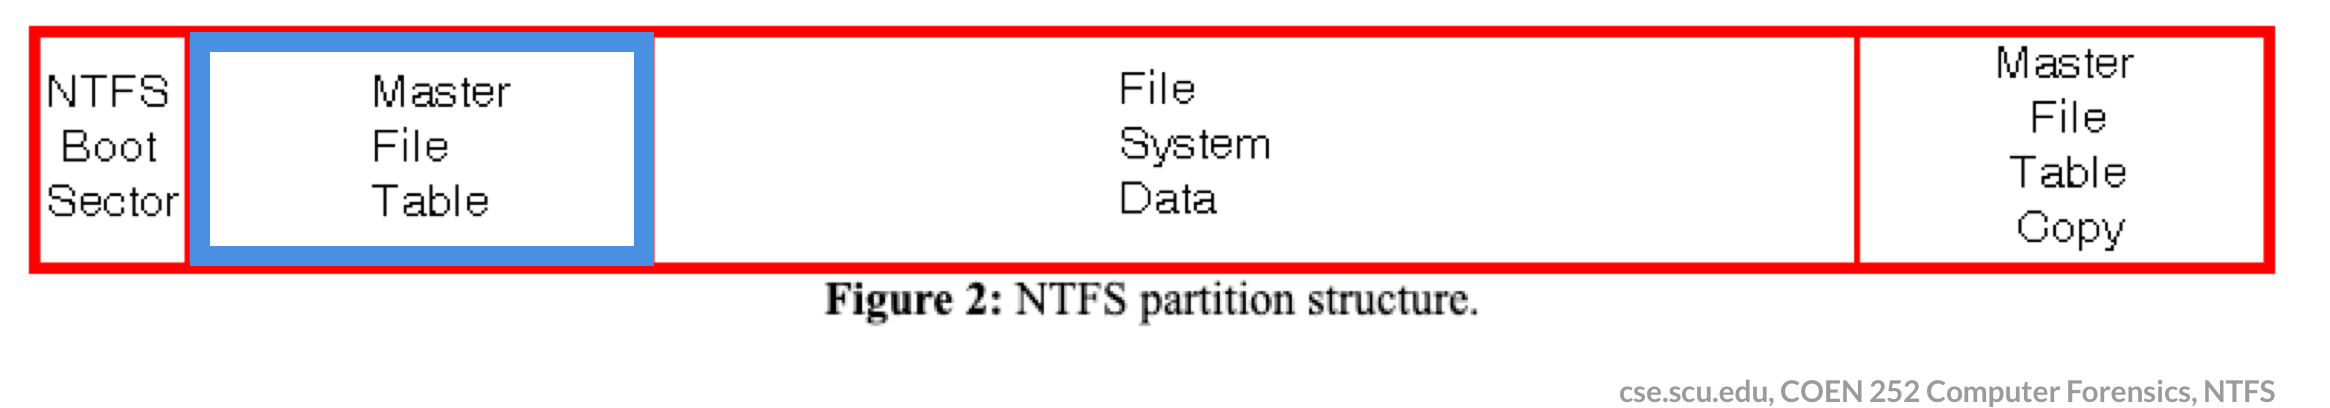
\includegraphics[width=\linewidth]{../images/week_9_notes_1_12.png}
    \end{center}

    \bigskip

    \underline{\textbf{Refernces:}}

    \bigskip

    \begin{enumerate}[1)]
        \item Webopedia : MFT - Master File Table, \href{https://www.webopedia.com/TERM/M/MFT.html}{link}
        \item Santa Clara University : COEN 252 Computer Forensics, \href{http://www.cse.scu.edu/~tschwarz/coen252_07Fall/Lectures/NTFS.html}{link}
    \end{enumerate}
    % \item MFT Record for a Small Directory
    % \item Better I/O performance through parallelism
\end{itemize}

\end{document}